%
% Explicación sobre redes Feistel, presentación de FPE.
% Proyecto Lovelace.
%

\subsection{Redes Feistel}

\begin{frame}{FFX}{Redes Feistel}

  \only<1>
  {
    \begin{figure}[H]
      \begin{center}
        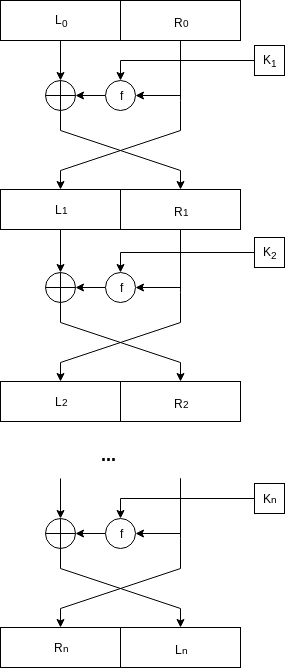
\includegraphics[height=0.7\textheight]
          {../../../diagramas_comunes/redes_feistel/feistel.png}
        \caption{Red Feistel, versión original.}
      \end{center}
    \end{figure}
  }

  \note<1>
  {
    Una de las características más importantes es que no se necesita una
    función de ronda inversa. La operación de descifrado se obtiene
    despejando, solamente. Por ejemplo, en una última instancia solamente se
    conoce $ L_n $ y $ R_n $:

    $$ R_{n-1} = L_n $$
    $$ L_{n-1} = f_{k_n}(R_{n-1}) \oplus R_n $$
  }

  \only<2>
  {
    \begin{figure}[H]
      \centering
      \begin{subfigure}{0.45\textwidth}
        \begin{center}
          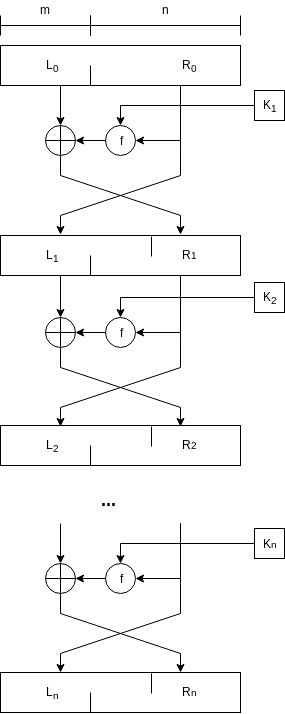
\includegraphics[height=0.65\textheight]
            {../../../diagramas_comunes/redes_feistel/desbalanceadas.png}
          \caption{Redes desbalanceadas.}
        \end{center}
      \end{subfigure}
      \begin{subfigure}{0.45\textwidth}
        \begin{center}
          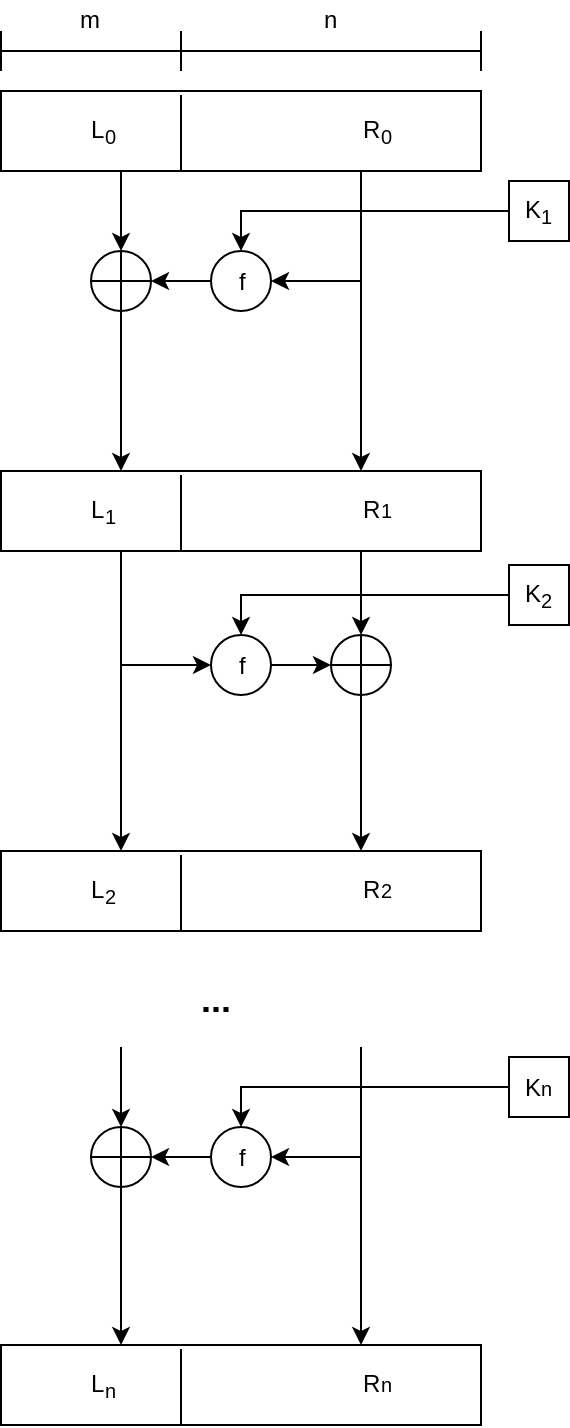
\includegraphics[height=0.65\textheight]
            {../../../diagramas_comunes/redes_feistel/alternantes.png}
          \caption{Redes alternantes.}
        \end{center}
      \end{subfigure}
      \caption{Generalizaciones de las redes Feistel.}
    \end{figure}
  }

  \note<2>
  {
    Puede haber distintos grados de desbalanceo. En caso de que este sea igual
    a cero, la red está balanceada (versión original).

    Las desbalanceadas llevan el costo extra de hacer la partición del bloque
    en cada ronda. Las alternantes necesitan de dos funciones de ronda.

    Después de terminar explicación, regresar a 1 y poner ejemplo con
    alfabeto binario y con alfabeto decimal. FFSEM estaba pensado para
    alfabetos binarios solamente, por lo que había que utilizar caminata
    cíclica en la función de ronda.
  }

  \only<3>
  {
    La operación de una red Feistel desbalanceada se puede resumir en las
    siguientes ecuaciones:
    \begin{align*}
      L_{i} &= R_{i - 1} \\
      R_{i} &= F_k(R_{i - 1}) \oplus L_{i - 1}
    \end{align*}

    Estas son las mismas que las de una red Feistel balanceada, con el costo
    extra de que en cada iteración hay que estar redistribuyendo los bloques.
  }

  \note<3>
  {
    El problema de estas es que hay que estar concatenando y volviendo a partir
    en cada iteración.
  }

  \only<4>
  {
    La operación de una red Feistel alternante se puede resumir en las
    siguientes ecuaciones:

    Si la ronda es par:
    \begin{align*}
      L_{i} &= F^1_k(R_{i - 1}) \oplus L_{i - 1} \\
      R_{i} &= R_{i - 1}
    \end{align*}

    Si la ronda es impar:
    \begin{align*}
      R_{i} &= F^2_k(L_{i - 1}) \oplus R_{i - 1} \\
      L_{i} &= L_{i - 1}
    \end{align*}
  }

  \note<4>
  {
    La implementación de estas es mucho más sencilla: no hay que hacer
    reparticiones en cada ronda; el proceso de cifrado y el de descifrado es
    prácticamente el mismo.
  }

\end{frame}

\begin{frame}{FFX}{Función de ronda}

  \only<1>
  {
    La función de ronda propuesta en \cite{ffx_2} es AES CBC MAC, aunque también
    puede ser usado cualquier otro cifrado por bloques o función hash.

    \begin{figure}[H]
      \begin{center}
        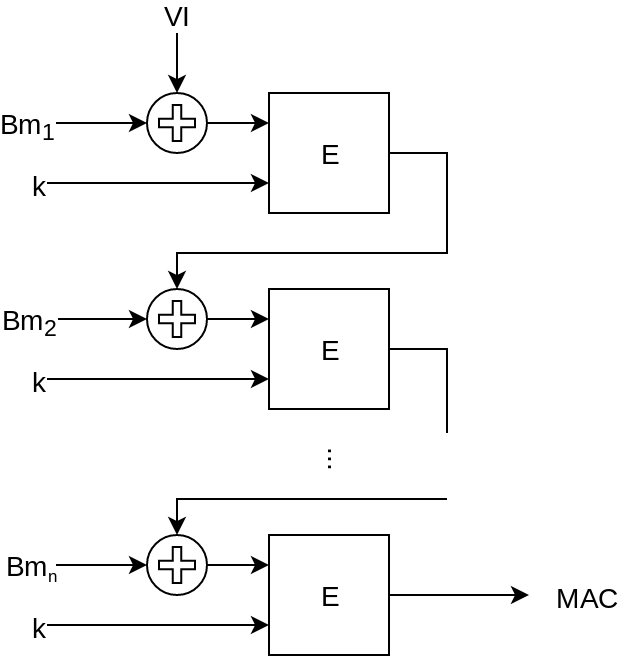
\includegraphics[height=0.35\textheight]{diagramas/cbc_mac.png}
        \caption{CBC MAC.}
      \end{center}
    \end{figure}

    La salida de la primitiva utilizada determina el tamaño del espacio de
    mensajes aceptado.
  }

  \note<1>
  {
    Esta última característica es lo que permite que FFX funciones sobre
    cadenas de cualquier longitud. Por ejemplo, se puede poner un cifrado
    de flujo en el lugar de la función de ronda.
  }

  \only<2>
  {
    La salida de la función de ronda se debe adaptar al alfabeto usado:

    \begin{itemize}

      \item En el caso de un alfabeto binario, tomar solamente el número
        de bits que la red Feistel requiere.

      \item En el caso de un alfabeto de caracteres, se debe interpretar de
        manera que produzca el número de caracteres necesarios. La forma más
        simple para hacer esto es tomar la salida de la primitiva módulo
        $ m^n $, en donde $ m $ es la cardinalidad del alfabeto y $ n $ el
        número de caracteres ocupados por la red.

        En \cite{ffx_2} se propone partir la salida de CBC MAC en dos: usar
        la primera mitad para producir $ n/2 $ caracteres, y la segunda
        mitad para los restantes.

    \end{itemize}
  }

  \note<2>
  {
    \textbf{TODO:} En el caso de los alfabetos de caracteres, ¿cuál es la
    diferencia en cuestión de seguridad entre uno y otro esquema? Creo que,
    el segundo es mejor, dado que toma en cuenta más bits de la salida de
    la primitiva.

    Antes de pasar a la siguiente sección, hablar de los \textit{tweaks} y
    de los números de rondas recomendados.
  }

\end{frame}
